\label{sec:TEO_FRAMEWORK}
%%%%%%%%%%%%%%%%%%%%%%%%%%%%%
In the early XIX century when Augustin-Jean Fresnel performed Thomas Young experiment, he proved empirically that light behaves like a wave. The results disproved the generally accepted corpuscular theory of light developed by Newton. This lead to the devolpment of a wave theory of light that ended up with Maxwell's equations \cite{maxwell1954electricity}. This set of 4 equations, describes how electromagnetic waves behave under any circumstance. \\

Few mathematical treatment is required to derive a wave equation that all electromagnetic waves must obey. The result 
\begin{equation}
    \frac{\partial^2 u}{\partial z^2} = \frac{1}{v^2}\frac{\partial^2 u}{\partial t^2},
    \label{eq:wave_eqn}
\end{equation}
 gives rise to a family of solutions that satisfy the super-position principle \footnote{The sum of two solutions to equation \ref{eq:wave_eqn} is also a solution to the wave equation.}. This principle, is the cornerstone that enable mathematics to describe the interaction of two light beams predicted by Young 220 years ago.  

\subsection{INTERFERENCE}
Interference is the phenomena associated to the sum of waves and the interaction of light itself. Thus, the work proceeds to define interference as the vector sum of the amplitudes of two light waves. Figure \ref{fig:BasicInterf} illustrates the sum of 3 sets of waves. The first row is called constructive interference where the amplitudes magnify each other. The second row is a visualization of destructive interference \footnote{Encountering annihilation in our models is not good for physicists because keep in mind that light is a natural system ruled by conservation laws. Thus, this case brings to question: what happens with that conservation of energy in a case of two light waves? Turns out, energy is simply distributed in a different configuration.}  where a maximum of a wave interferes with a minimum of the other canceling each other out. The last row is a case that is nether total constructive nor destructive interference. \\

\begin{figure}[H]
    \centering
    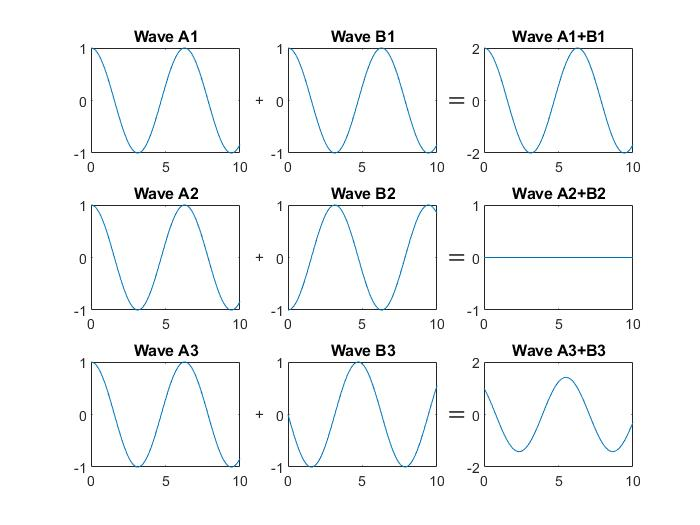
\includegraphics[scale=0.30]{Figures/Figures_I/Basic_Interference.jpg}
    \caption{1) Constructive Interference of A and B, 2) Destructive interference of A and B, 3) Partial constructive interference of A and B. }
    \label{fig:BasicInterf}
\end{figure}

It is important to mention that a series of characteristics have to hold for a optical system to interfere. To further understand these considerations, consider the vector sum of two light waves:  $\Vec{E_1}=E_1 exp(i[\vec{k_1}\cdot \vec{r}-wt+\epsilon_1])$ and $\Vec{E_2}=E_2 exp(i[(\vec{k_2}\cdot \vec{r}-wt+\epsilon_2])$. The resulting sum, averaged over time \footnote{This measurable quantity is calculated by taking a mean value over time of the energy of the field. This leads to the relation $I = \langle E \cdot E \rangle$} is
\begin{equation}
    I_{tot} = I_1 + I2 + 2 cos(\delta),
    \label{eq:interf}
\end{equation}
where $\delta = (\vec{k_2}-\vec{k_1})\cdot \vec{r} + (\epsilon_1-\epsilon_2)$. Result \ref{eq:interf} hints at the fact that $w, k, E_i$ and polarization play a critical role in that collectively create the phenomena of interference. The characteristics are summarized as follows. For electromagnetic waves to interact they must: 
\begin{itemize}
    \item be monochromatic.
    \item be coherent (temporal coherence). 
    \item share a polarization state.
\end{itemize}

Figure \ref{fig:VectorInterf} is an excellent visualization of this result.However in a macroscopic characterization, the important takeaway is that the directional difference between  $\vec{k_1} $ and $\vec{k_2}$ controls the number of fringes in displayed in figure \ref{fig:Interf_Types}. 

\begin{figure}[H]
    \centering
    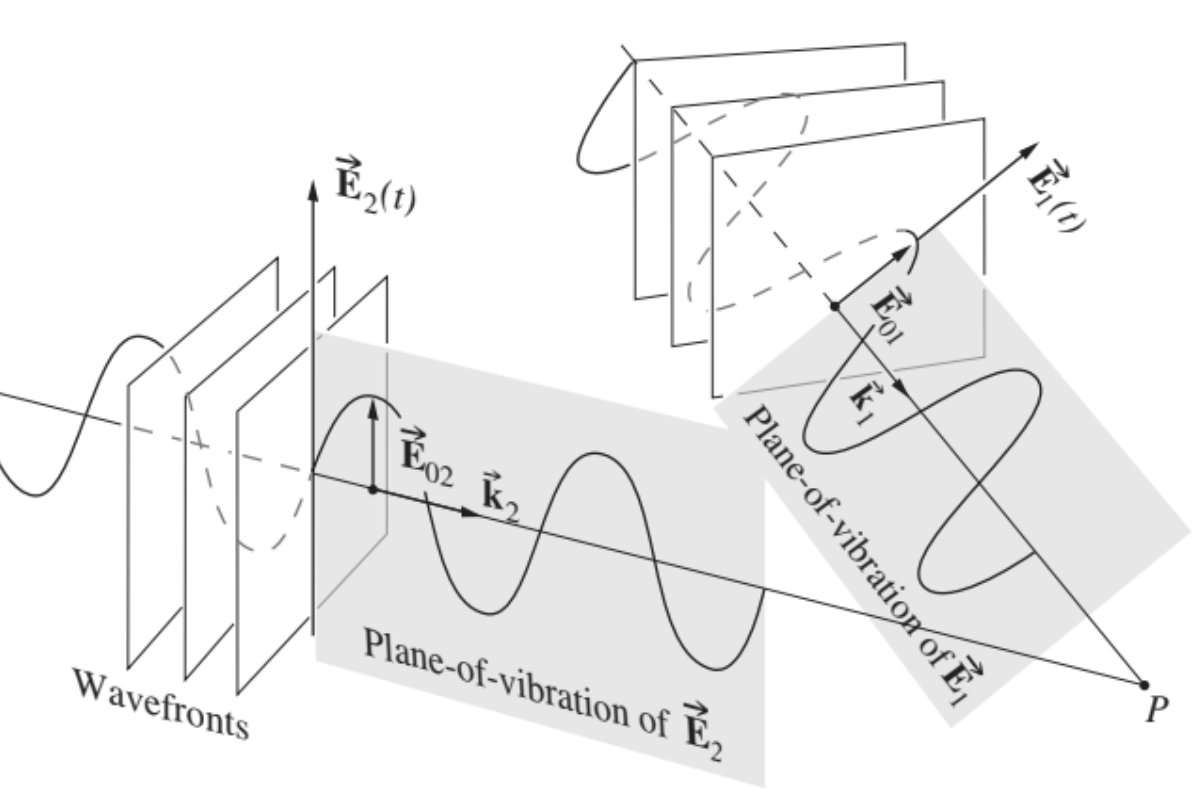
\includegraphics[scale=0.30]{Figures/Figures_I/Vectorsum_Interference.png}
    \caption{Vector Sum of two electromagnetic waves \cite{hecht1987optics}}
    \label{fig:VectorInterf}
\end{figure}

%%%%%%%%%%%%%%%%%%%%%%%%%%%%%
\subsection{TEMPORAL COHERENCE}
The measurement of coherence is a comparison between the relative phases of two light waves \cite{guenther2015modern}. As of 2021 every realistic source of light has an associated bandwidth of temporal frequencies. This means that for the case of our LASER is not perfectly monochromatic. The implications of this fact permits us to invoke Heisenberg uncertainty principle 
\begin{equation} 
\Delta E \Delta t\ge \hbar/2 ,
\end{equation} 
Where $\hbar$ is Planks constant. The size of this bandwidth is related to $\Delta E$ and temporal coherence($\tau$) is related to $\Delta t$. The key takeaway is that for more monochromatic beams more temporal coherence they are allowed to have. 

The mathematical analysis of such statement can be done with Fourier transforms. It all borrows down to introducing the mutual coherence function ($\gamma$)
\begin{equation}
 \gamma (\tau) = \frac{\Gamma(\tau)}{\Gamma(0)},
\end{equation}
where 
\begin{equation}
 \Gamma (\tau) = \int_0^{\infty} E_0(\tau)^2 exp(-iw\tau) dw,
\end{equation}
relates bandwidth with coherence ($\tau$). Also note the last results is a Fourier transform. 

%%%%%%%%%%%%%%%%%%%%%%%%%%%%%
\subsection{INTERFEROMETERS}
In the most general sense, any interferometer works by either dividing its wavefront or its amplitude. In the case of wavefront division, a point-like source emits a wave and a physical barrier is applied to filter only some selected parts of the wavefront (Figure \ref{fig:Interf_Types} A). Then, these resulting parts of the wavefront interfere with each other. In the case of amplitude division, a beam splitter (a dielectric) splits an incident beam into two by reflecting some amplitude and transmitting the rest of the amplitude (Figure \ref{fig:Interf_Types} B). Later it is possible to design a optical system that lets this two beams interfere with each other. 

\begin{figure} [H]
    \centering
    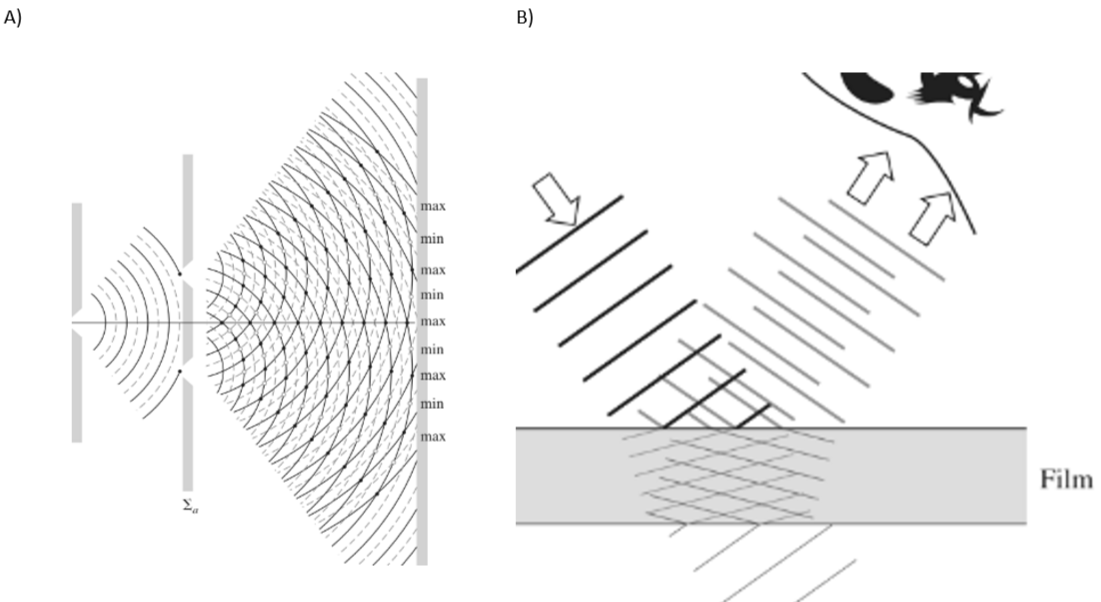
\includegraphics[width=.30\textwidth]{Figures/Figures_I/Interferometers_Types.png}
    \caption{General principles of interferometers \cite{hecht1987optics}.}
    \label{fig:Interf_Types}
\end{figure}

Thomas Young´s experiment discussed at the beginning of this section was a interferometer of wavefront division. However, in this work we will be using a type of amplitude division interferometer called Mach Zehnder. This later interferometer splits a beam into two amplitudes in a ratio of 50-50. Then the two beams travel independent paths to later be collimated to create interference.

%%%%%%%%%%%%%%%%%%%%%%%%%%%%%
